\documentclass{article}
\usepackage[utf8]{inputenc}
\usepackage{amsmath}
\usepackage{amsthm}
\usepackage{graphicx}
\usepackage{geometry}
\usepackage{caption}
\usepackage{minted}
\usemintedstyle{tango}
\geometry{a4paper, portrait, margin=1in}

\theoremstyle{plain}
\newtheorem{thm}{Theorem}

\theoremstyle{definition}
\newtheorem{defn}{Definition} % definition numbers are dependent on theorem numbers
\newtheorem{exmp}{Example} % same for example numbers

\title{Operating Systems (UE18CS302) \\
    \large Unit 1}
\author{Aronya Baksy}
\date{August 2020}

\begin{document}

\maketitle

\section{What is an Operating System}
    \begin{defn}
        A system program that acts as an intermediary between user and the computer hardware being used.
    \end{defn}
    
    \subsection{Goals of an OS}
    
        \begin{enumerate}
            \item Execute user programs, make problem solving easier for the user
            
            
            \item Make the system convenient to use
            
            \item Use computer hardware resources in the most efficient manner possible
        \end{enumerate}
        
        User convenience and optimized resource usage most of the time are contradictory goals, which involves a trade-off to achieve the optimum balance. 
    
    \subsection{The User's view of an OS}
    The end user of a computer system defines the Operating System in the following manner:
    
    \begin{itemize}
        \item Offers \textbf{convenient} access to computational power, while being \textbf{easy to use} and offering \textbf{good performance}
        
        \item The end user does not care much about actual resource usage in the computer.
    
    \end{itemize}
    
    The user level definition of an OS may even vary based on the computation environment.
    
    \begin{itemize}
        \item Workstations and mainframe computers must share server resources fairly among all users.
        
        \item A handheld system is resource poor and must be optimized for high battery life and ease of use
        
        \item An embedded system or an IoT device does not have any User Interface (UI) and must be optimized for a specific task only. 
    \end{itemize}
    
    \subsection{The system view of an OS}
    
    From the point of view of actual computing, the OS may be defined as the following
    
    \begin{itemize}
        \item The OS is a \textbf{resource manager}. It allocates the computing resources in a fair and efficient manner to all programs that request for access to these resources. 
        
        \item The OS is a \textbf{control program}. It controls the execution of programs and prevents errors/improper use of the computing resources by these programs.
    \end{itemize}
    
    \subsection{Definition of an OS}
    
    The OS may be defined from either the system or user POVs. Hence there are no fixed definitions of an OS. \\
    The following are two loose and intuitive definitions that may be used:
    \begin{itemize}
        \item "All the software shipped by a vendor while selling an operating system": this defn is suitable for a program like Microsoft Windows that is sold as a single unit comprising of application and system software.
        
        \item "A kernel program that runs at all times on a computer system": this defn is suitable for OSes belonging to the UNIX and Linux families that are available only as kernels without any extra application software on top. 
    \end{itemize}

\section{Computer System Organization}

A computer consists of hardware resources which are to be managed by the OS.\\
A program known as the \textbf{bootstrap} program (stored in read-only memory) initializes all the aspects of the system (CPU registers, I/O Devices) on startup/reboot, and loads the actual kernel of the OS to start execution.\\
Once the kernel is loaded and executing, it can start providing services to the system and its users. Some services are provided outside of the kernel, by system programs that are loaded into memory at boot time to become system
processes.\\
Once this phase is complete, the system is fully booted, and the system waits for some event to occur.

\subsection{Interrupts}

An event occurrence is defined by a signal known as an \textbf{interrupt}.\\
An interrupt is a signal provided by a peripheral device to the CPU requesting for some access to the CPU's computation to serve its needs.\\
When an interrupt is received by the CPU, it transfers control to the appropriate \textbf{Interrupt Service Routine} (ISR) which is a function in the OS that handles the functionalities of that device specifically.\\
The \textbf{Interrupt Vector Table} (IVT) stores the address of the ISR corresponding to each type of device.\\
An \textbf{exception} is a software generated interrupt that is raised upon an error or at the request of the user.\\
The following mechanisms are involved in handling of Interrupts
\begin{itemize}
    \item Storing the current PC and register values before interrupt was received by CPU
    \item Interrupt handling methods: 
    \begin{enumerate}
        \item \textbf{Polling:} Read the state (busy/available) of each I/O device in a list and then service the one who makes a request. Repeat continuously while CPU has power. 
        
        \item \textbf{Vectored Interrupts:} The device notifies the CPU that it needs attention. The CPU reads the address of the appropriate ISR from the IVT and pauses the current program execution to handle the ISR. 
    \end{enumerate}
\end{itemize}

\begin{figure}[ht]
    \centering
    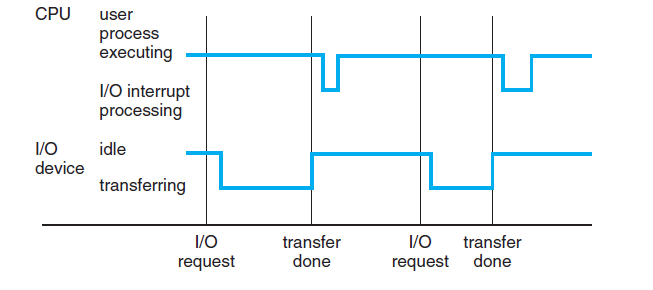
\includegraphics[scale=0.6]{os2.png}
    \caption{Interrupt Timeline for a single process}
    \label{fig:my_label1}
\end{figure}

\subsection{CPU}

\begin{itemize}
    \item $\geq 1$ CPUs, along with I/O device controllers that exist on a single bus to access the shared memory.  
    
    \item CPUs and I/O devices compete for memory access cycles. 
    
    \item The I/O devices and CPUs execute \textbf{concurrently}
\end{itemize}

\begin{figure}[h]
    \centering
    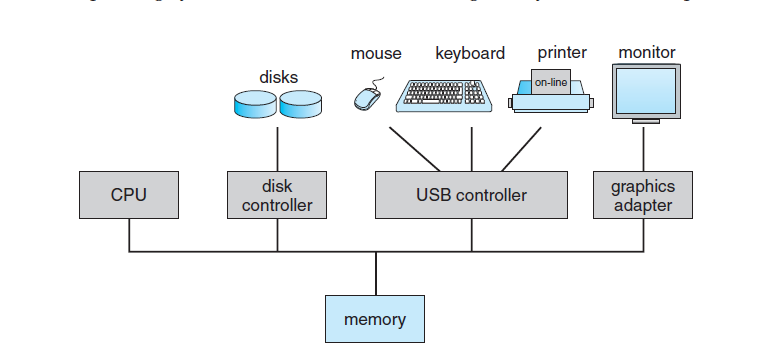
\includegraphics[scale=0.85]{os1.png}
    \caption{Hardware Resource Organization}
    \label{fig:my_label}
\end{figure}

\subsection{Storage:}

Every computer has the following levels of storage in it's hierarchy.

\begin{enumerate}
    \item \textbf{Main Memory:} Volatile in nature, random access
    
    \item \textbf{Secondary Memory:} Large capacity, non volatile and acts as an extension to the main memory. This is used for permanent storage of user data \& programs.
\end{enumerate}
In addition, the CPU contains its own \textbf{cache} and \textbf{registers} that are used to reduce the number of memory accesses to the slower main/secondary memories and hence improve CPU performance.\\

\section{Computer System Architecture}
The following is a categorization of different system architectures based on the number of general-purpose processors they use

\subsection{Singe Processor System}

\begin{itemize}
    \item A single general-purpose CPU executes a general-purpose instruction set, including instructions from \textbf{user processes.}
    
    \item Single processor systems may contain other processing units which are special purpose units. They may be device specific controllers (I/O devices) or I/O management processors that move data rapidly between components (typically found on mainframes).
    
    \item The special purpose processors run a very limited and specific instruction set, and they cannot run user process instructions.
    
    \item Sometimes, they are managed by the operating system, in that the operating system sends them information about their next task and monitors their status.
    
    \item In other cases, these processors function entirely autonomously, without the involvement of the OS.
\end{itemize}

\subsection{Multiprocessor System}

\begin{itemize}
    \item These are also called \textbf{parallel} or \textbf{multicore} systems.
    
    \item Such systems have two or more processors in close communication, sharing the computer bus and sometimes the clock, memory, and peripheral devices.
    
    \item Multiprocessing architecture has the following advantages:
    
    \begin{itemize}
        \item Increased Throughput
        
        \item Economies of scale
        
        \item Increased reliability
    \end{itemize}
    
    \item \textbf{Increased reliability} is an important advantage in performance critical industry applications. 
    
    \item \textbf{Graceful degradation} is a property of multiprocessing systems where the failure of a certain proportion of the total hardware resources results in only a proportional drop in performance.
    
    \item Some systems go beyond graceful degradation and are called \textbf{fault tolerant}, because they can suffer a failure of any single component and still continue operation. Fault tolerance requires a mechanism to allow the failure to be detected, diagnosed, and, if possible, corrected.
    
    \item Two main types of multiprocessing systems are in use nowadays. 
    \begin{itemize}
        \item \textbf{Asymmetric multiprocessing:} Each processor is assigned a separate, specific task, with a single \textit{boss} processor handling the functioning of all the others. 
        
        \item \textbf{Symmetric multiprocessing:} Each processor is capable of performing all the tasks on the system. All processors are peers (there is no boss-worker relationship). Each processor maintains its own set of registers and local private cache, but a shared main memory common to all processors exists. 
        
        \begin{figure}[h]
            \centering
            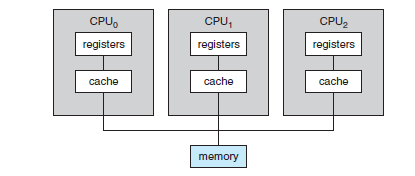
\includegraphics{os3.png}
            \caption{Symmetric Multiprocessing Architecture}
            \label{fig:my_label_3}
        \end{figure}
    \end{itemize}
    
    \item Some concerns in symmetric architectures arise from load distribution (one CPU idle, another one working at high load is undesirable), and I/O management (make sure the data reaches the right processor). These concerns are resolved by the sharing of certain data structures among all the processors.
    
    \item The following memory access models exist in Multiprocessing systems
    \begin{itemize}
        \item \textbf{UMA:} Uniform Memory Access, meaning all CPUs take exactly the same time for a memory access (read/write) to the RAM.
        
        \item \textbf{NUMA:} Non-Uniform Memory Access, meaning some parts of memory take longer to access than other parts (this leads to performance penalties). 
    \end{itemize}
    
    \item In contrast to multi-chip systems where each CPU is a discrete silicon wafer, the recent trend is towards \textbf{multi-core} systems where all the CPUs are organized on a single silicon wafer.
    
    \item Multicore architectures have the benefit of faster inter-CPU communication (intra chip vs inter chip) and lower power consumption (single chip vs multiple chips). 
    
    \item All multicore systems are multiprocessor systems, but all multiprocessor systems are not multicore systems.
    
    \item \textbf{Blade servers} are systems in which multiple
processor boards, I/O boards, and networking boards are placed in the same chassis. The difference between these and traditional multiprocessor systems is that each blade-processor board boots independently and runs its own operating system. Some blade-server boards are multiprocessor as well, which blurs the lines between types of computers. In essence, these servers consist of multiple independent multiprocessor systems.
\end{itemize}

\begin{figure}[h]
    \centering
    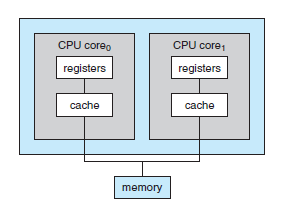
\includegraphics{os4}
    \caption{Multi-core Architecture (dual core)}
    \label{fig:my_label_4}
\end{figure}

\subsection{Clustered Systems}

\begin{itemize}
    \item These consist of multiple systems called \textit{nodes} connected to each other.
    
    \item Each node may be a single processor or a multiprocessor system. 
    
    \item The generally accepted definition of clustered systems is that they share a common memory and are connected by an interconnect protocol like LAN or InfiniBand.
    
    \item The main application of clustered systems is in \textbf{high-availability} scenarios, where the service delivery must continue even when one or more nodes fail. This is done by building in various redundancies into the system. A software layer monitors all the clusters, and in case one node fails, the node that monitors can take up the memory and tasks done by the failed node and resume them. 
    
    \item Clustered systems may be organized as follows
    \begin{itemize}
        \item \textbf{Asymmetric:} One machine is in \textbf{hot-standby} mode while another runs an application. In case of failure of the latter, the former takes on the role of the active system. 
        
        \item \textbf{Symmetric:} $\geq 2$ hosts run applications and monitor each other simultaneously. This is a more efficient architecture but it needs more than 1 app to be run at a time. 
    \end{itemize}
    
    \item For an application to take advantage of the \textbf{high-performance computing (HPC)} environment afforded by a cluster, it must be explicitly parallelized. 
    
    \item This is done by splitting the program into independent tasks that function separately on individual nodes,  and a final combination of all the individual results from each task.
    (eg: the MapReduce framework in Hadoop)
    
    \item Memory concurrency and the avoidance of conflicting operations being carried out by different nodes on the shared memory is managed by a hardware called the \textbf{Distributed Lock Manager (DLM)}
\end{itemize}

\begin{figure}
    \centering
    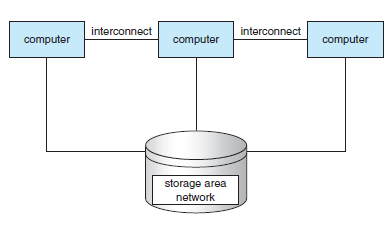
\includegraphics{os5.png}
    \caption{Clustered System Architecture}
    \label{fig:my_label_5}
\end{figure}

\section{Structure of an Operating System}

\begin{itemize}
    \item \textbf{Multiprogramming} is a paradigm that allows the CPU to always have atleast one job to do (in terms of either I/O device handling or user program handling) 
    
    \item The multiprogramming algorithm works as follows:
    \begin{itemize}
        \item The OS maintains a job pool consisting of all processes residing on the disk that are awaiting access to the main memory. 
        \item The set of jobs that are actually in main memory is a subset of this job pool. The OS picks a job and begins to execute it.
        
        \item While this job waits (for an I/O operation) a non-multiprogrammed OS might have made the CPU sit idle too.
        
        \item But in a multiprogramming envt, the OS switches to another job during this wait time and executes it. 
        
        \item When this job needs to wait, the CPU switches to another job and starts running it, and so on. 
        
        \item Eventually the first job finishes waiting and it gets back its control of the CPU. 
        
        \item As long as at least one job needs to execute, the CPU is never idle. 
    \end{itemize}
    
    \item Multiprogramming systems only handle effective use of all the hardware resources, but they do not handle the user interaction with all these hardware resources. 
    
    \item The \textbf{timesharing model} is a logical extension of multiprogramming, in which the CPU switches between various jobs at a very fast rate, and the switches occur so frequently that the users can interact with each program while it is running.
    
    \begin{itemize}
        \item Time sharing OSes need an interactive system, where the user can directly communicate with the system hardware using I/O devices like a mouse, keyboard and display.
        
        \item This necessitates a short response time - less than 1 second
        
        \item A time-shared OS allows multiple users to access a single computer, where each user submits a job and the computer executes between all the jobs for some time interval each. 
        
        \item Choosing which job to load into memory when all the possible jobs cannot fit is the job of a set of algorithms called \textbf{job scheduling} algorithms.
    \end{itemize}
    
    \item In a time-sharing system, the operating system must ensure reasonable response time. This goal is sometimes accomplished through \textbf{swapping}, whereby processes are swapped in and out of main memory to the disk. 
    
    \item A more common method for ensuring reasonable response time is \textbf{virtual memory}, a technique that allows the execution of a process that is not completely in memory. 
    
    \item The main advantage of the virtual-memory scheme is that it enables users to run programs that are larger than actual physical memory. Further, it abstracts main memory into a large, uniform array of storage, separating logical memory as viewed by the user from physical memory. This arrangement frees programmers from concern over memory-storage limitations.
    
    \item Time Sharing OSes must also provide a file system, a disk management to manage the physical aspects of the file system, a resource protection mechanism from inappropriate use, as well as mechanisms for job synchronization and communication, to prevent jobs from getting stuck in a deadlock waiting for each other.
\end{itemize}

\section{Operating System Operations}
The OS must ensure that problems/errors occurring in a user program are localized only to that program, and do not affect any of the other processes running on the CPU.\\
Not doing so may lead to explicit errors (like the interruption of other processes) or more subtle errors (like one program erroneously overwriting the data of another).\\
Multi-mode operation of OSes, with the requisite hardware support is one approach to solve this problem.
\subsection{Dual Mode Operation}
\begin{itemize}
    \item The two modes of operation are the \textbf{user mode} and the \textbf{kernel mode} (also known as the \textbf{supervisor mode}, \textbf{system mode}, or the \textbf{privileged mode}). 
    
    \item A \textbf{mode bit} in hardware indicates the current mode of operation (1-user mode, 0-kernel mode)
    
    \item The mode bit distinguishes between applications run on behalf of the user (user mode) and on behalf of the system (kernel mode). 
    
    \item The system boots up into kernel mode by default. After the OS is loaded, it switches into user mode and executes user jobs. Traps/interrupts cause the OS to switch into kernel mode from user mode. 
    
    \item The system transitions from user mode to kernel mode whenever the user makes a system call (ie. a request for a system functionality). Before passing the control back to the user program, the mode bit is switched to 1 (user mode) again. 
    
    \item The Dual mode operation allows for protecting the system hardware from errant users, and for protecting errant users from each other. 
    
    \item Certain machine instructions, ie. those with the potential to harm the system, are designated as \textbf{privileged instructions} and can be executed only in kernel mode. These include the instruction to switch to kernel mode, as well as I/O control instructions, timer management and interrupt management. 
\end{itemize}

\subsection{Multi Mode Operation}

\begin{itemize}
    \item Multi mode operation allows other functions such as \textbf{Virtual Machine Management (VMM)} to be implemented in the OS. This is indicated by a separate mode in CPUs that support virtualization.
    
    \item In such a case, the mode is indicated by $> 1$ bit.
    
    \item The VMM is at a privilege level above the user but below the kernel, which is needed to change the CPU state while creating virtual machines. 
\end{itemize}

We can now see the life cycle of instruction execution in a computer system. Initial control resides in the operating system, where instructions are executed in kernel mode. When control is given to a user application, the mode is set to
user mode. Eventually, control is switched back to the operating system via an interrupt, a trap, or a system call.

\begin{figure}
    \centering
    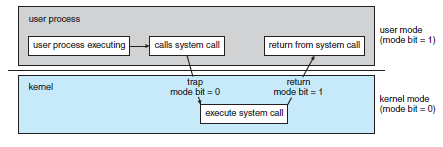
\includegraphics{os6.png}
    \caption{Switching between User and Kernel modes}
    \label{fig:my_label_6}
\end{figure}

\subsection{System Calls}

\begin{itemize}
    \item System calls provide the means for a user program to ask the operating system to perform tasks reserved for the operating system on the user program’s behalf.
    
    \item A system call usually takes the form of a trap to a specific location in the interrupt vector. This trap can be executed by a generic trap instruction or a specific instruction (as in the MIPS ISA)
    
    \item When a system call is executed, it is typically treated by the hardware as a software interrupt. 
    
    \item Control passes through the interrupt vector to a service routine in the operating system, and the mode bit is set to kernel mode.
    
    \item The system-call service routine is a part of the operating system. The kernel examines the interrupting instruction to determine what system call has occurred; a parameter indicates what type of service the user program is requesting.

    \item Additional information needed for the request may be passed in registers, on the stack, or in memory (with pointers to the memory locations passed in registers)
    
    \item The kernel verifies the validity of the request format, executes the request, and returns control to the next instruction after the system call.
\end{itemize}

Without the protection of dual mode operation, catastrophic results may arise where a user program overwrites the system's data (eg: MS-DOS running on early Intel x86 chips like the 8086 and 8088, modern x86 chips provide dual mode op.)

\subsection{System Timer}
\begin{itemize}
    \item The job of the timer is to make sure that the user program returns control to the OS after a specific time period, so that the system can return to kernel mode. 
    
    \item The timer is set to interrupt the computer after either a fixed delay or a variable delay. 
    
    \item \textbf{Variable timers} are implemented using the system clock in combination with a down counter. 
    
    \item Before turning over control to the user, the operating system ensures that the timer is set to interrupt. If the timer interrupts, control transfers automatically to the operating system, which may treat the interrupt as a fatal error or may give the program more time. Clearly, instructions that modify the content of the timer are privileged.
\end{itemize}

\section{Computing Environments}

\subsection{Traditional Computing}

\begin{itemize}
    \item Traditional computing model consists of multiple individual workstation PCs connected to a single network with servers providing file storage and printing services. 
    
    \item In the modern era, this has been replaced by an infrastructure where mobile computers as well as Desktops can connect to the company's internal network using a \textbf{portal}. 
    
    \item Mobile computers can also use cellular or wireless networks using the company portal for further portability of information. 
    
    \item Even in the home environment, now there is a prevalence of fast internet speeds, with more access to data. Many homes use personal \textbf{firewalls} to protect their networks from security breaches.
    
    \item In contrast to the time sharing approach between users, modern desktops/laptops/servers/mobile computers provide time sharing between multiple processes owned by the same owner (eg: multiple windows open by one user)
\end{itemize}

\subsection{Mobile Computing}
\begin{itemize}
    \item Traditional mobile systems sacrificed processing power, screen size and memory capacity in exchange for portability. 
    
    \item In modern mobile systems, this is no longer the case, with mobiles now being able to provide functions that are not possible or impractical on a desktop (eg: GPS navigation, gyroscope related functions, etc.)
    
    \item The wide range of apps that run on mobile devices are made possible by a large number of specialized \textbf{sensors} that are a part of mobile systems (eg: GPS, gyroscope, ambient light sensors, advanced camera systems, optical fingerprint sensors, AR sensors).
    
    \item Mobile systems use the IEEE 802.11 protocol (commonly called WiFi) or cellular data (3G/4G/5G protocol) to access the internet. 
    
    \item Google's \textbf{Android} and Apple's \textbf{iOS} (formerly called iPhone OS) are the major players in this segment.
\end{itemize}

\subsection{Distributed Computing}
\begin{itemize}
    \item A distributed system is a collection of physically separate, possibly heterogeneous computer systems that are networked together to provide users with access to shared resources. 
    
    \item Network access may be generalized as a form of file access, or as a separate protocol with network functions. 
    
    \item There are various different of networks based on their range. They are \textbf{LAN} (room/building/campus range), \textbf{WAN} (building/city/country range), \textbf{MAN} (intra city), \textbf{PAN} (personal device range). 
    
    \item Network transmission media also vary, such as copper cables, fiber optic cables, and wireless methods (microwave/radio wave/IR communication).
    
    \item A \textbf{network operating system} is an operating system that provides features such as file sharing across the network, along with a communication scheme that allows different processes on different computers to exchange messages. 
    
    \item A computer running a network operating system acts autonomously from all other computers on the network, although it is aware of the network and is able to communicate with other networked computers.
    
    \item A distributed operating system provides a less autonomous environment. The different computers communicate closely enough to provide the illusion that only a single operating system controls the network.
\end{itemize}

\subsection{Client-Server Computing}
\begin{itemize}
    \item Instead of a centralized architecture (where multiple terminals access the compute resources of a single mainframe), the functionalities handled by the mainframe systems are now being handled by PCs themselves, through a web interface. 
    
    \item This necessitates that many of the systems be \textbf{servers}, which satisfy the requests made by \textbf{clients} over the internet. 
    
    \item Servers can be classified into:
    \begin{itemize}
        \item \textbf{Compute-Server systems:} The server executes the action requested by the server and returns the result to the client. (eg: DB servers)
        
        \item \textbf{File-Server systems:} The server provides a file system interface where the client can create, update, delete and read files. (eg: web server using HTTP)
    \end{itemize}
    
    \begin{figure}[h]
        \centering
        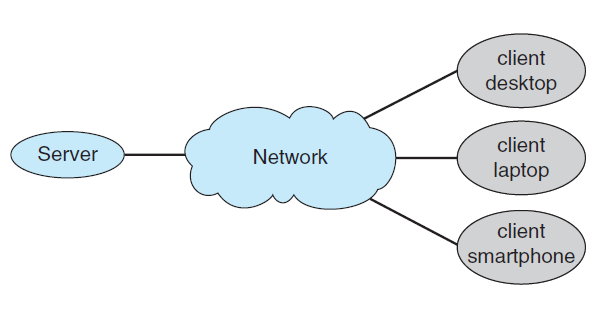
\includegraphics[scale=0.8]{os7.png}
        \caption{Client-Server architecture}
        \label{fig:my_label_7}
    \end{figure}
\end{itemize}

\subsection{Peer-to-Peer Computing (P2P)}
\begin{itemize}
    \item All nodes in a P2P system are considered to be peers, and each may act as a client or server depending on whether it requests or provides some service.
    
    \item In a client-server system, the total system performance depends on the server (ie. the server is a bottleneck) but in a P2P system services can be provided by >1 distributed nodes. 
    
    \item Once a new node joins the peer network, it determines what services are available in the following ways:
    \begin{itemize}
        \item The new node registers itself on a specialized \textit{lookup service} on the network. A node that desires a service must find it on this lookup service and then make the request to the appropriate peer node. 
        
        \item The node that desires a service can broadcast its request to all the nodes in the network, and the appropriate node sends a response to this request (the rest of the nodes may ignore it). This approach needs a \textit{discovery protocol} to allow a peer to discover the services offered by its fellow peers on the network. 
    \end{itemize}
    
    \item File sharing services such as Napster (centralized lookup table), Gnutella (broadcast file request to all nodes) and the BitTorrent client are examples of P2P systems. Skype is another example of a P2P client sending voice messages over the internet using a protocol called VoIP.
    
    \begin{figure}[h]
        \centering
        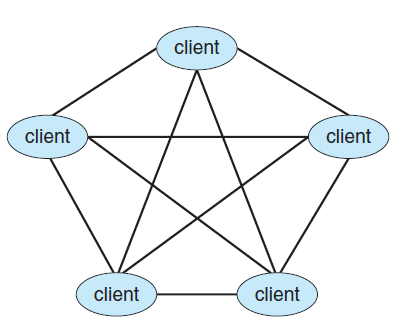
\includegraphics[scale=0.6]{os8.png}
        \caption{A peer-to-peer system with no centralized service}
        \label{fig:my_label_8}
    \end{figure}
\end{itemize}

\subsection{Virtualization}
\begin{itemize}
    \item Virtualization is a technology that allows operating systems to run as applications within other operating systems.
    
    \item Broadly speaking, virtualization is one member of a class of software that also includes \textbf{emulation}.
    
    \item \textbf{Emulation} is used when the source and target OSes are written for different CPU architectures. (eg: Apple's Rosetta for applications compiled on PowerPC architecture to run on Intel x86 CPUs, and Rosetta 2 for applications compiled on Intel x86 to run on ARM CPUs)
    
    \item That same concept can be extended to allow an entire operating system written for one platform to run on another. Emulation comes at a heavy price, however. Every machine-level instruction that runs natively on the source system must be translated to the equivalent function on the target system, frequently resulting in several target instructions. 
    
    \item If the source and target CPUs have similar performance levels, the emulated code can run much slower than the native code.
    
    \item In \textbf{Virtualization}, an OS natively compiled for one CPU architecture runs within another OS compiled for the same CPU architecture. 
    
    \item On laptops and desktops, a VMM allows the user to install multiple operating systems for exploration or to run applications written for operating systems other than the native host.
    
    \begin{figure}[h]
        \centering
        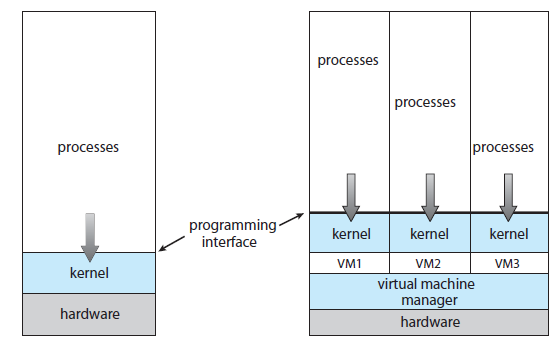
\includegraphics{os9.png}
        \caption{Architecture of the VMWare Virtual Machine}
        \label{fig:my_label_9}
    \end{figure}
\end{itemize}

\subsection{Cloud Computing}
\begin{itemize}
    \item Cloud computing is a type of computing that delivers computing, storage, and even applications as a service across a network. 
    
    \item In some ways, it is a logical extension of virtualization, because it uses virtualization as a base for its functionality. 
    
    \item For example, the Amazon Elastic Compute Cloud (EC2) facility has thousands of servers, millions of virtual machines, and petabytes of storage available for use by anyone on the Internet. Users pay as per their usage of these services.
    
    \item The various types of cloud computing are as follows:
    \begin{itemize}
        \item \textbf{Public cloud:} A cloud available via the internet for anyone willing to pay.
        
        \item \textbf{Private Cloud:} A cloud run by a company for its internal use
        
        \item \textbf{Hybrid Cloud:} A cloud that includes both public and private components.
        
        \item \textbf{SaaS:} Applications available over the internet (eg: Google Office Suite)
        
        \item \textbf{PaaS:} A software stack ready for application use over the internet (eg: a DB server)
        
        \item \textbf{IaaS:} Servers/storage hardware available over the internet (eg: Google Cloud Storage solutions like BigTable, FireStore etc.)
    \end{itemize}
    
    \begin{figure}[h]
        \centering
        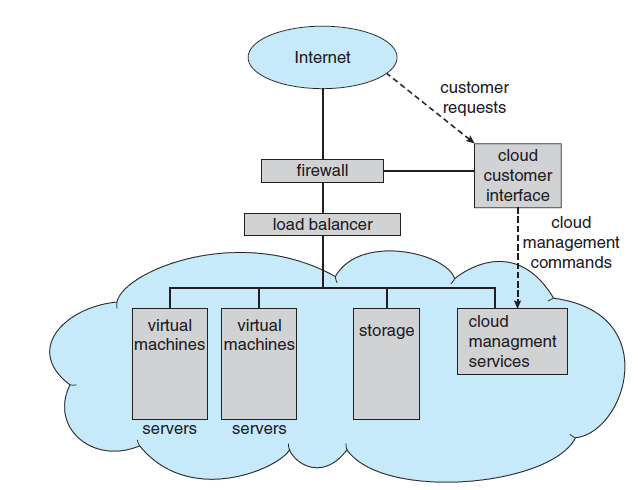
\includegraphics[scale=0.8]{os10.png}
        \caption{Cloud Computing (IaaS)}
        \label{fig:my_label_10}
    \end{figure}
\end{itemize}

\subsection{Real-Time Operating Systems}

\begin{itemize}
    \item Embedded systems are hardware devices with very specific purposes, and have little or no user interface for humans.
    
    \item They may be general purpose computers running standard OSes like Linux, special purpose devices running device specific OSes (network infrastructure like link-layer switches and routers), or even Application Specific Integrated Circuits (ASICs) which do not need an OS.
    
    \item A real-time OS is used when strict time constraints are placed on the processing/data flow. Data brought in from sensors is used to modify the surrounding environment in real time. 
    
    \item A real time OS is said to function correctly only if the result is returned within the given time constraints. 
\end{itemize}

\section{Operating System Services}
\subsection{User Services}
\begin{itemize}
    \item \textbf{User Interface:} This may take three forms, a Command Line Interface (CLI) which relies on text-based individual commands that are run (eg: Linux), a batch OS where commands are entered into files which are executed (eg: bat files in Windows, Shell scripts in Linux OSes), or a Graphical User Interface (GUI) which uses familiar visual controls to enable the user to access OS functions (eg: Windows, Linux distros having GNOME/KDE desktop)
    
    \item \textbf{Program Execution:} The ability to load an user program from memory, execute it and terminate it (normally or abnormally).
    
    \item \textbf{I/O Management:} Manage the functionality of various I/O devices which the user is not allowed to do themselves (because of security reasons).
    
    \item \textbf{File system manipulation:} Read and write files, Create/Update/Delete/Search for files in the file system. Permission and access management for certain files.
    
    \item \textbf{Communication:} Inter Process Communication, which may be implemented via shared memory between processes, or using a message passing system between 2 or more processes, where communication takes place by means of packet transmission between processes. 
    
    \item \textbf{Error Detection:} CPU/Memory errors, I/O device errors, user errors. Take appropriate action as per error type, and ensure correct and consistent computing. 
\end{itemize}

\subsection{System Services:}
\begin{itemize}
    \item \textbf{Resource Allocation:} Resource allocation to all users/jobs running at a given instant in time. Some resources (CPU cycles, main memory, file storage) have a specific allocation code, while others (such as I/O devices) have a more general request and release code. 
    
    \item \textbf{Accounting:} Keeping track of resource usage type, grouped by user. Such statistics are used for billing in cloud instances and for system optimization by system admins.
    
    \item \textbf{Protection and Security:} Protection means ensuring that all access to system resources is controlled (processes don't overwrite each other's memory, interfere with each other's execution). Security means protection of system resources and data from outside intruders, by requiring user login with a password, and also the defense of I/O and network devices from illegal access attempts. 
\end{itemize}
\begin{figure}[h]
    \centering
    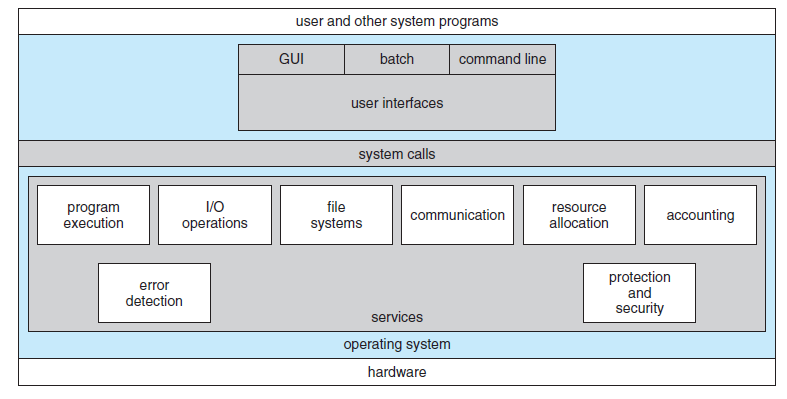
\includegraphics{os11.png}
    \caption{OS Services Architecture}
    \label{fig:my_label_11}
\end{figure}

\section{Operating System Design and Implementation}
The user and system goals defined above are the main driving forces behind design of a new operating system. These, along with any application specific requirements (like in the field of embedded systems) guide the design process of an OS.
\subsection{Policy and Mechanism}
\begin{itemize}
    \item The \textbf{separation of policy and mechanism} is an important paradigm of software development. 
    
    \item The policy is an idea of \textit{what} is to be done, while the mechanism is \textit{how} that policy will be done. (eg: the design of the system timer is a mechanism decision, but the timer delay is a policy decision)
    
    \item The two must be separated as policies may change, and without a clear separation while developing the OS, a change in policy will result in needing to overhaul large parts of the source code. 
    
    \item On the other hand, developing a policy independent mechanism means that if policies do change later, only a certain number of parameters will have to be changed in order for the OS to function according to the new policy. 
    
    \item Microkernel based OSes (like QNX, developed by BlackBerry for embedded systems) take this philosophy to its logical extreme, by implementing only a basic set of building blocks, which the user can combine to give more advanced functionalities to the OS.
    
    \item Consumer OSes like Windows and Mac OS X have a very tight integration between mechanism and policy to enforce a global look and feel to the OS. 
\end{itemize}

\subsection{Implementation}
\begin{itemize}
    \item Operating Systems consist of various modules written by many different teams of people over a long time, hence there is little scope of generalizing the implementation of an OS.
    
    \item Most early OSes were written exclusively in assembly instructions. 
    
    \item Nowadays, high-level languages like C or even C++ are used. The choice of these 2 languages is their closeness to the system hardware. 
    
    \item Modern OSes are more often than not in many different languages. Low level kernel modules are written in assembly, while higher level routines may be written in C, system software in C/C++ and application programs in ultra high level scripting or interpreted languages like Python, Java or PERL. 
    
    \item The first system that was not written in assembly language was probably
the Master Control Program (MCP) for Burroughs computers. MCP was written
in a variant of ALGOL. MULTICS, developed at MIT, was written mainly in
the system programming language PL/1.
\end{itemize}

\section{Processes}

\subsection{The concept of a Process}
    \begin{defn}
    A process is defined as a program under execution. 
    \end{defn}
\begin{itemize}
    
    \item A process is more than the source code of the program that it was created from. The following are the components of a process.
    \begin{enumerate}
        \item \textbf{Text/Program Code:} Source code of the program that generated the process
        
        \item \textbf{Program Counter, Process Registers:} These identify the current activity of the process. 
        
        \item \textbf{Stack:} A temporary data store for function parameters, local variables and function return addresses.
        
        \item \textbf{Global Data:} For all global and static variables
        
        \item \textbf{Heap:} Space for all memory allocated by the process at runtime
    \end{enumerate}
    
    \item Although two processes may be associated with the same program, they are nevertheless considered two separate execution sequences. 
    
    \item For instance, several users may be running different copies of the mail program, or the same user may invoke many copies of the web browser program. 
    
    \item Each of these is a separate process; and although the text sections are equivalent, the data, heap, and stack sections vary. 
    
    \item It is also common to have a process that spawns many processes as it runs. 
\end{itemize}
\begin{figure}[ht]
    \centering
    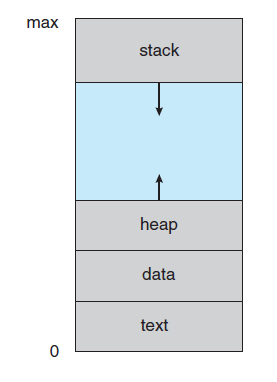
\includegraphics{os12.png}
    \caption{A process in Memory}
    \label{fig:my_label_12}
\end{figure}

\subsection{Process States}
\begin{itemize}
    \item \textbf{New:} Process is being created
    
    \item \textbf{Running:} Process instructions are being executed
    
    \item \textbf{Waiting:} Process is waiting for an I/O operation or memory access. 
    
    \item \textbf{Ready:} The process is waiting to be assigned to a processor. 
    
    \item \textbf{Terminated:} The process has finished execution. 
\end{itemize}

\begin{figure}[h]
    \centering
    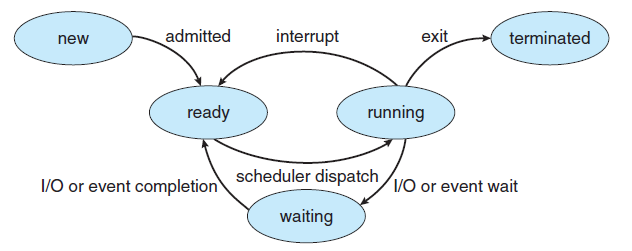
\includegraphics{os13.png}
    \caption{State Transition Diagram for a Process}
    \label{fig:my_label_13}
\end{figure}

\subsection{Process Control Block (PCB)}
\begin{itemize}
    \item A PCB (also called a \textbf{task control block}) holds all the information that the CPU needs to identify and manage a process. The information held in a PCB is:
    \begin{enumerate}
        \item \textbf{Process State:} One of the 5 states described above
        
        \item \textbf{Program Counter:} Address of the next instruction to execute. 
        
        \item \textbf{CPU Registers:} These vary by platform architecture, but in general they include accumulators, index registers,
        stack pointers, and general-purpose registers, plus any condition-code
        information. \\
        Along with the program counter, this state information must
        be saved when an interrupt occurs, to allow the process to be continued
        correctly afterward
        
        \item \textbf{Scheduling Info.:} Pointers to process queues, process priority
        
        \item \textbf{Memory Management Info.:} This information may include such
        items as the value of the base and limit registers and the page tables, or the
        segment tables, depending on the memory system used by the operating
        system
        
        \item \textbf{Accounting Info.:} CPU hours and real time hours used, time limits, account numbers, job or process numbers
        
        \item \textbf{I/O Device Info.:} List of all I/O devices allocated to the process, list of all files accessed by the process. 
    \end{enumerate}
\end{itemize}

\subsection{Threads}
\begin{itemize}
    \item Threads allow processes to perform multiple tasks at the same time
    
    \item All the threads belonging to a particular process share the same address space but have different program counters of their own.
    
    \item On multi core machines, threads can run in parallel, improving process performance.
\end{itemize}

\subsection{Process Scheduling}
To meet the objectives of multiprogramming and time sharing, the process scheduler selects tasks from a pool of processes and loads them into the main memory for exxecution. 
\subsubsection{Scheduling Queues}
\begin{itemize}
    \item As processes enter the system, they enter the \textbf{job queue}, which is a queue of all processes in the system.
    
    \item The scheduler selects processes from the job queue to enter the \textbf{ready queue}, which signifies loading the process into the main memory and preparing it for execution.
    
    \item A separate queue, called the \textbf{device queue} is maintained to list all processes that are waiting for I/O access or disk access.
\end{itemize}
\begin{figure}[ht]
    \centering
    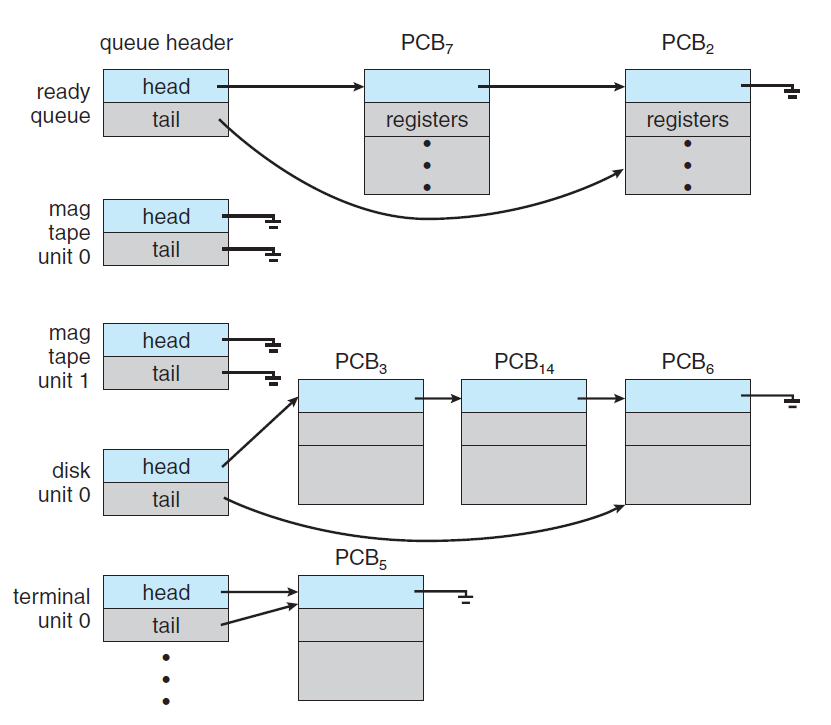
\includegraphics[scale=0.45]{os15.png}
    \caption{Ready Queue and various device queues}
    \label{fig:my_label_xxx}
\end{figure}

\subsubsection{Process Schedulers}
\begin{itemize}
    \item There are three main types of schedulers that operate, the \textbf{long-term}, \textbf{short-term} and \textbf{medium term} schedulers.
    
    \item The \textbf{long-term scheduler}, or the job scheduler, selects processes from the job pool on the disk, and loads them into memory to make them ready for execution.
    
    \item The \textbf{short-term scheduler}, or CPU scheduler, selects one process from the ready processes and allocates the CPU to it.
    
    \item The short-term scheduler executes more frequently than the long term scheduler, at around once every 100ms. 
    
    \item Speed is of the essence in a short-term scheduler. If 10ms are needed to schedule a process that executes for 100ms, then $\frac{10}{100+10} = 9.09\%$ of CPU time is wasted in scheduling. 
    
    \item The long term scheduler operates much less frequently, around once every few minutes. The long term scheduler controls the \textbf{degree of multiprogramming} (the number of processes in memory). 
    
    \item For a stable degree of multiprogramming, the rate of process creation and the rate of process departure from the system must be equal. Thus, the long-term scheduler may need to be invoked only when a process leaves the system.
    
    \item The long-term scheduler must select a good \textit{process mix} of \textbf{CPU-bound} processes (that spend more time on computation than on I/O operations) and \textbf{I/O bound} processes (that spend more time on I/O access than on computation). 
    
    \item If all the processes are I/O bound, the ready queue will always be empty and the short term scheduler will have nothing to do.
    
    \item If all the processes are CPU bound, then the I/O waiting queue will be always empty and the I/O devices will be unused. 
    
    \item The \textbf{medium-term scheduler} is used to \textit{reduce} the degree of multiprogramming by swapping out a waiting process from memory to the disk, and reloading it to the memory once it's wait is over. This process is called \textit{swapping}.
    
    \item Swapping may be necessary to improve the process mix or because
a change in memory requirements has overcommitted available memory,
requiring memory to be freed up.
\end{itemize}

\begin{figure}[ht]
    \centering
    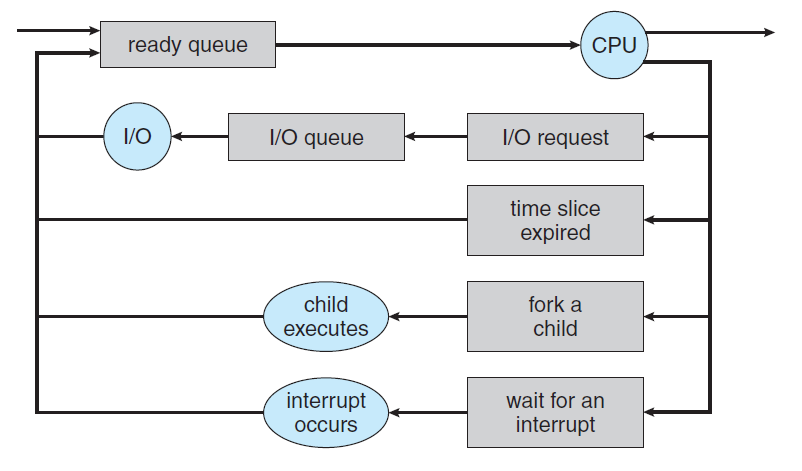
\includegraphics[scale=0.7]{os16.png}
    \caption{Queues in Process Scheduling}
    \label{fig:my_label_yy}
\end{figure}

\begin{figure}
    \centering
    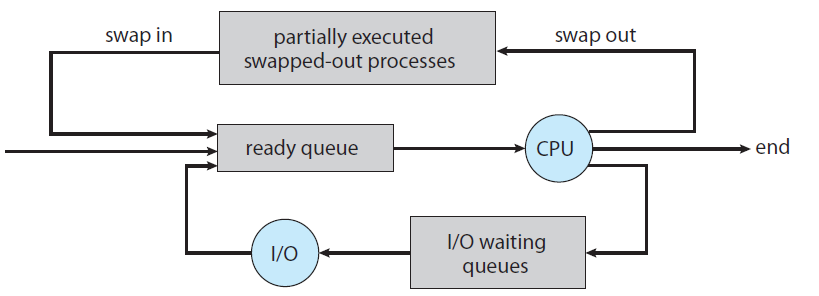
\includegraphics[scale=0.6]{os17.png}
    \caption{Medium-term Scheduling}
    \label{fig:my_label_yyx}
\end{figure}

\subsection{Context Switching}
\begin{itemize}
    \item An interrupt may cause the CPU to pause the execution of the current process and move to kernle model to execute a system call.
    
    \item In such a case, the \textbf{context} of the running process (represented by its Process Control Block or PCB) must be saved so that it can be later retrieved. 
    
    \item Switching the current context of the CPU involves a \textbf{state store} of the current running process, and a \textbf{state restore} of another process. 
    
    \item When a context switch occurs, the kernel saves the context of the old process in its PCB and loads the saved context of the new process scheduled to run.
    
    \item The address space of the process also needs to be saved, to prevent another process from overwriting the data in the old process that was stored away. 
    
    \item The time required for Context switching is purely an overhead, as no useful work is done at this time. It depends on hardware support, and greater OS complexity leads to larger context switching time. 
\end{itemize}

\begin{figure}[ht]
    \centering
    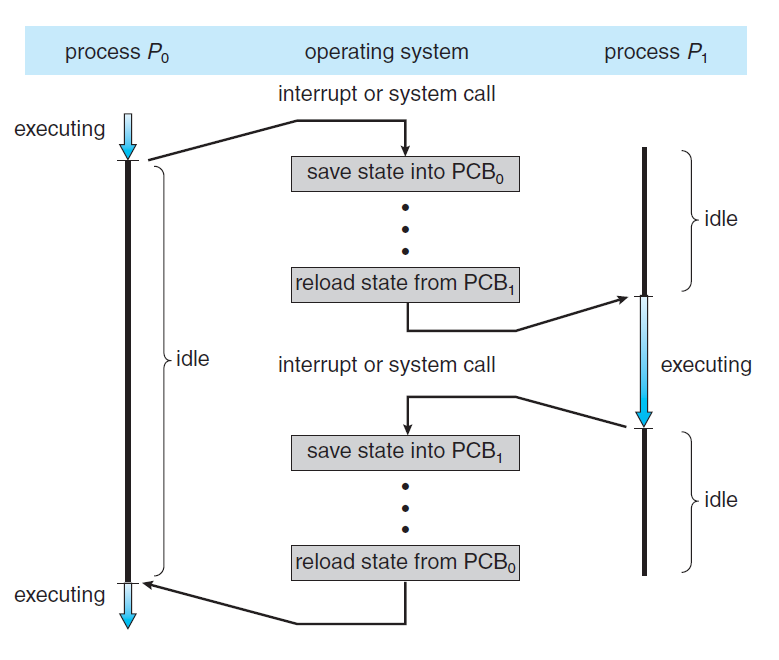
\includegraphics[scale=0.6]{os14.png}
    \caption{Context Switching from Process to Process}
    \label{fig:my_label_xx}
\end{figure}

\section{Process Operations}
\subsection{Process Creation}
\begin{itemize}
    \item A process, while executing, may create processes of its own. Such a situation leads to the creation of a \textbf{process tree}.
    
    \item In Linux, processes are identified by their \textbf{process identifier} (pid), which is an integer number. 
    
    \item The \texttt{init} process is the root process for all user processes. It's children are the \texttt{sshd} (used to manage users logging in via SSH) and the \texttt{kthreadd} (used to create additional processes that perform tasks on behalf of the kernel) processes. 
    \item A child process of a parent may be constrained to use only a subset of the parent's resources (CPU time, I/O devices, memory files), or it can directly obtain these from the OS.
    
    \item Restricting a child process to a subset of the parent’s resources prevents any process from overloading the system by creating too many child processes.
    
    \item There are two possibilites for execution when a child process is created:
    \begin{enumerate}
        \item Parent and child continue to execute concurrently
        
        \item Parent waits for some/all of its children to terminate.
    \end{enumerate}
    
    \item In terms of address space, the following possibilities exist:
    \begin{enumerate}
        \item Child is duplicate of parent (same data and program as parent)
        
        \item Child process has a new program loaded into it.
    \end{enumerate}
\end{itemize}
\begin{figure}[h]
    \centering
    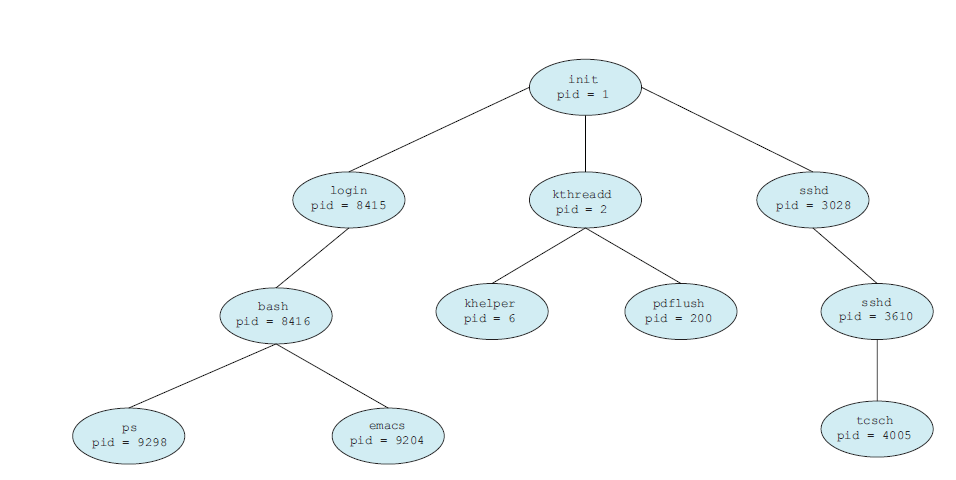
\includegraphics[scale=0.8]{os18.png}
    \caption{A Linux Process tree}
    \label{fig:my_label_z}
\end{figure}
\break
\begin{listing}[ht]
\centering
    \begin{minted}{c}
    
    #include<stdio.h>
    #include<unistd.h>
    #include<sys/types.h>
    #include<sys/wait.h>
    int main()
    {
        pid_t process_code;
        process_code = fork();
        
        if(process_code < 0) /* An error occurred */
        {
            fprintf(stderr, "Error occurred while forking\n");
            return 1;
        }
        else if(process_code == 0) /* child process */
        {
            execlp("/bin/ls", "ls", NULL);
        }
        else  /* Parent process waits for child process to finish */
        {
            wait(NULL);
            printf("Child process completed!\n");
        }
        return 0;
    }
    \end{minted}
    \title{Process creation using \texttt{fork} system call in UNIX}
\end{listing}
\begin{itemize}
    \item The \texttt{fork} call is used to create a copy of the current (orginal)process address space. This allows easy communication between parent and child processes.
    
    \item The return code of the \texttt{fork} call is 0 for the child process, and the non-zero pid of the child process is returned to the parent process. 
    
    \item After \texttt{fork()} creates a new process, the \texttt{exec()} system call is used to replace the process' memory space with a new program, and execute it. 
\end{itemize}
\begin{figure}[h]
    \centering
    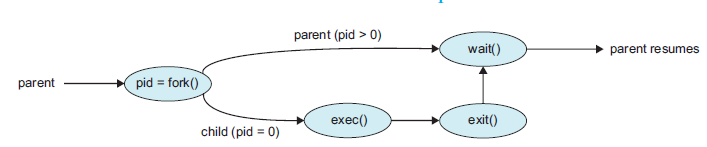
\includegraphics{os19.png}
    \caption{Process Creation using the \texttt{fork()} call}
    \label{fig:my_label_zzz}
\end{figure}

\subsection{Process Termination}
\begin{itemize}
    \item A process terminates when the last instruction is executed and it asks the OS to terminate it using the \texttt{exit()} call. 
    
    \item At this point, the process returns a status code to its parent using the \texttt{wait()} call, and the resources allocated to the process are deallocated. 
    
    \item Only parents can kill their child processes, using the appropriate identifier. This can be for the following reasons:
    \begin{itemize}
        \item Child using excess resources
        
        \item Child process task is no longer needed
        
        \item Parent is exiting, and OS doesn't allow child to run without its parent.
    \end{itemize}
    
    \item \textbf{Cascading termination} is the OS' mechanism to terminate a process, by recursively killing off all its child processes first.
    
    \item Parent processes wait for the termination of their children by issuing a \texttt{wait()} system call. The \texttt{wait()} call allows the parent to know the exit status of its children and to know the pid of the child process that terminated. 
    
    \item Until the parent of a process calls \texttt{wait()}, the terminated process must have an entry in the process table (as the exit status is contained in this entry). A process that has terminated but whose parent has not yet called \texttt{wait()} is called a \textbf{zombie} process.
    
    \item All processes briefly enter a zombie state when they state, as there is some delay between termination and the parent calling \texttt{wait()}.
    
    \item If the parent terminates instead of issuing a \texttt{wait()} call, the child processes become \textbf{orphan} processes. In UNIX and UNIX-like systems, this is handled by assigning the \texttt{init} process to be the parent of all the orphans. 
    
    \item The \texttt{init} process periodically invokes \texttt{wait()}, thereby allowing the exit status of any orphaned process to be collected and releasing the orphan’s pid.
\end{itemize}

\section{Process Scheduling}
\begin{itemize}
    \item While one process waits for some device or I/O response, the scheduler loads one more process to keep the CPU busy in the meantime. 
    
    \item Such an arrangement increases the level of multiprogramming, and keeps the CPU busy at all times, with no idle periods of inefficiency. 
    
    \item The success of this arrangement is due to the fact that processes commonly alternate between periods of heavy CPU activity (a \textbf{CPU burst}) and periods of high I/O activity (an \textbf{I/O burst}). 
    
    \item The frequency distribution of CPU and I/O bursts (CPU bound progs have few long CPU bursts, I/O bound progs have many short CPU bursts, and vice versa for I/O bursts) is important when choosing an appropriate scheduling algorithm.
\end{itemize}

\subsection{Preemptive and Non Preemptive Scheduling}

\begin{itemize}
    \item CPU scheduling takes place in the following four situations:
    \begin{enumerate}
        \item Process switching from \textbf{running} to the \textbf{waiting} state, for an I/O or memory access, or invocation of wait() for child process termination. 
        
        \item Process switching from \textbf{running} to \textbf{ready}, when an interrupt occurs.
        
        \item Process switching from \textbf{waiting} to \textbf{ready} state, for example when an I/O op. completes.
        
        \item Process \textbf{terminates}
    \end{enumerate}
    
    \item The situations 1 and 4 come under the purview of \textbf{non-preemptive} or \textbf{cooperative} scheduling. 
    
    \item Situations 2 and 3 come under \textbf{preemptive} scheduling. 
    
    \item Under non-preemptive scheduling, once a process is allocated the CPU, it takes control of the CPU until it has to wait or it terminates. 
    
    \item Preemptive scheduling can lead to race conditions. If one process is preempted while it is writing to some data location, and the new process reads from that location, then that data is an inconsistent state. 
    
    \item Preemptive scheduling can also affect kernel design. If a kernel process is preempted while it is changing some kernel data (eg: an I/O queue), then chaos ensues. UNIX family OSes solve this problem by waiting for the entire system call or I/O op to complete before performing the context switching. This is a working solution but is not feasible in real time OSes. 
    
    \item The \textbf{dispatcher} gives control of the CPU to the process that is selected by the short term scheduler. This involves a context switch, a switch to user mode, and jumping to the appropriate location in the user program to start execution. 
    
    \item Every process switch invokes the dispatcher, and the time taken for the dispatcher to stop one process and start another is called the \textbf{dispatch latency}.
\end{itemize}

\subsection{Scheduling Criteria}
\begin{itemize}
    \item \textbf{CPU Utilization:} The fraction of time the CPU is kept busy. Theoretically can be anywhere from 0 to 100\%, but real world values range from 40\% to 90\%.
    
    \item\textbf{Throughput:} Number of processes completed per unit time. 
    
    \item \textbf{Turnaround Time:} Interval between process submission and process completion. Turnaround time is the sum of the periods spent waiting to get into memory, waiting in the ready queue, executing on the CPU, and doing I/O.
    
    \item \textbf{Waiting Time:} Sum of all time periods spent by process in the wait queue.
    
    \item \textbf{Response Time:} Time between process submission and first response. 
\end{itemize}

\textbf{maximize:} CPU Util, Throughput\\
\textbf{minimize:} Turnaround time, wait time, response time

\subsection{Scheduling Algorithms}

\subsubsection{First Come First Serve (FCFS) Scheduling}
\begin{itemize}
    \item Processes are added to the ready queue in the order in which they arrive. 
    
    \item The average wait times for FCFS depend very heavily on the process mix, and the burst times for each process. A long process arriving behind many short ones can lead to short wait time, but a long process in front of short ones may lead to longer wait times. 
    
    \item The effect of a long process in front of many short processes, making the short processes wait for CPU time, is called the \textbf{convoy effect}.
    
    \item The FCFS is non preemptive because it allocates CPU time entirely to the new process, and it causes problems in time sharing systems where each user must get CPU time at regular intervals.
\end{itemize}

\subsubsection{Shortest Job First (SJF) Scheduling}
\begin{itemize}
    \item The process with the shortest CPU burst time is selected for CPU time. 
    
    \item To predict the length of the next CPU burst, in a long term system the process time limit per user can be used, which is supplied by the user. 
    
    \item For a short term scheduling situation, the next CPU burst time is predicted using an exponential average of the previous CPU burst times.
    
    \begin{equation}
        \tau_{n+1} = \alpha t_n + (1-\alpha) \tau_{n}
    \end{equation}
    
    Where $\tau_{i}$ refers to the \textit{predicted} CPU burst value at the time index $i$, and $t_i$ refers to the \textit{actual} CPU burst time at time index $i$.
    
    \item The parameter $\alpha$ is chosen to be a constant with value $< 1$, most often a value of 0.5
    
    \item The preemptive version of SJF, also called shortest waiting-time first, where the process with the shortest CPU burst time is chosen, and the current process is pre-empted in its place. 
\end{itemize}

\subsubsection{Priority Scheduling}
\begin{itemize}
    \item Each process is associated with a priority (a non-negative integer) and the CPU is allocated to the process with the highest priority.
    
    \item Allocating priorities to processes can be due to external or internal reasons. 
    
    \item Internal factors could be user time limits, memory requirements, the number of open files, and even the ratio of average I/O and CPU burst times. 
    
    \item External factors are primarily influenced by human considerations of process importance. 
    
    \item Priority scheduling may be preemptive (if the priority of the incoming process is higher than that of the currently running process then the currently running process is preempted), or non-preemptive (if the incoming process has a higher priority than the currently running one, it is placed at the head of the ready queue).
    
    \item Low priority processes may be blocked from CPU access by a steady stream of high priority processes arriving constantly. This problem is called \textbf{starvation}.
    
    \item The problem of starvation is resolved by a process called\textbf{aging}, wherein the priority of a waiting process is increased after fixed intervals of time. 
\end{itemize}

\subsubsection{Round Robin Scheduling}
\begin{itemize}
    \item The fundamental unit of time in an RRS algorithm is called the \textbf{time slice} or \textbf{time quantum} (denoted as $q$).
    
    \item Each process is assigned a time equal to $q$ on the CPU, and the ready queue is treated as a circular queue. Once all processes in the queue have got one $q$ unit of CPU time, the allocation circles back to the first process in the ready queue.
    
    \item No process has a wait time of more than $(n-1)q$ where $n$ is the number of processes on the ready queue. Every process gets an allocation of $1/n$ of the CPU time.  
    
    \item The system timer is rigged to throw an interrupt and cause a context switch after every quantum of time. 
    
    \item A very small value of $q$ can lead to large overheads due to frequent context switching, while a large value of $q$ can lead to the RRS algorithm becoming a FCFS system instead.
\end{itemize}

\subsubsection{Multilevel Queue Scheduling}
\begin{itemize}
    \item When processes can be classified into groups (eg: \textbf{foreground} (interactive) and \textbf{background} (batch) processes), the MQS scheduling is used. 
    
    \item The groups would each have different scheduling requirements, and one group (foreground) would have an externally defined priority over the other. 
    
    \item The MQS algorithm partitions the ready queue into several smaller queues, each with its own scheduling algorithm and associated properties. 
    
    \item The processes are permanently assigned to one queue, generally based on some property of the process, such as memory size, process priority, or process type.
    
    \item Between queues, there could be an ordering of queues such that processes in one queue have higher priority over processes in another queue. 
    
    \item An alternative approach to inter-queue scheduling is to have a time slice of the CPU for each queue to submit processes to the CPU. (eg: foreground queue gets 80\% of CPU time, and background queue gets 20\%)
\end{itemize}

\begin{figure}[t]
    \centering
    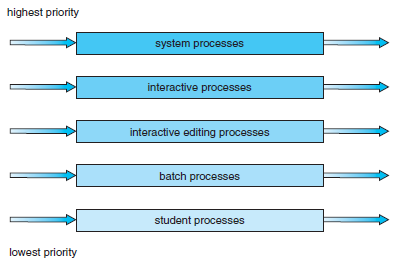
\includegraphics{os20.png}
    \caption{Multilevel Queue Scheduling}
    \label{fig:my_label_zzzzz}
\end{figure}

\subsubsection{Multilevel Feedback Queue Scheduling}
\begin{itemize}
    \item This allows processes to move between all the various process queues, with the intent of separating processes according to their CPU burst times. 
    
    \item If a process uses too much of CPU time, it may be moved to a lower-priority queue, with I/O bound and interactive processes in the highest priority queues. 
    
    \item To prevent the problem of starvation, aging is implemented in this algorithm by moving a process to a higher priority queue. 
    
    \item A Multilevel Feedback Scheduling algorithm is characterized by:
    \begin{enumerate}
        \item The number of queues, and their individual scheduling algorithms
        
        \item The method used to promote or demote a process from one queue to another
        
        \item The method used to determine which queue an incoming process will enter when it needs service. 
    \end{enumerate}
\end{itemize}
\begin{figure}[h]
    \centering
    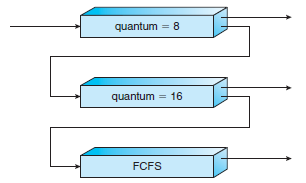
\includegraphics{os21.png}
    \caption{Multilevel Feedback Queue Scheduling}
    \label{fig:my_label_xws}
\end{figure}


\section{Multiprocessor Scheduling}
\subsection{Approaches}
\begin{itemize}
    \item The \textbf{asymmetric} multiprocessing approach involves one master CPU that manages all scheduling, I/O and system activites while the rest execute only user code.
    
    \item Only one processor needs to access the data structures for scheduling, hence data sharing and concurrency problems are fewer here. 
    
    \item In a \textbf{symmetric} multiprocessor, each processor is self scheduling, with each having either its own ready queue or a shared ready queue, but each having their own scheduling algorithms. 
    
    \item SMP systems having common data structures must ensure concurrency and 
\end{itemize}
\subsection{Processor Affinity}
\begin{itemize}
    \item Processor affinity is the phenomenon where a process perfers to execute on one particular processor. 
    
    \item There are two types: \textbf{soft affinity} implies that the system tries to keep the process on that processor, but will migrate it if needed, while \textbf{hard affinity} allows the process to specify a subset of the processors on which it will execute. 
    
    \item Affinity allows for performance improvement via caching, as keeping a process on one processor allows for its data to be present in cache, hence reducing memory accesses to main memory. 
    
    \item In boards with NUMA memory, the scheduler and memory placement algos work together such that processes using one particular processor are allocated memory that is faster to access for that processor. 
\end{itemize}

\subsection{Load Balancing}
\begin{itemize}
    \item In order to ensure that most processors does not remain idle while only one works extra hard to handle all processes, load balancing is important. This is implemented by moving processes between queues. 
    
    \item \textbf{Push migration} involves a specific task that checks all the CPUs and moves tasks from overloaded CPUs to idle ones. \textbf{Pull migration} occurs when idle CPUs pull processes from overloaded CPUs. 
    
    \item Load balancing nullifies the performance gain derived from processor affinity via caching, as each migration involves invalidating the old CPUs cache and copying those values to the new CPU. 
\end{itemize}

\subsection{Multicore Scheduling}
\begin{itemize}
    \item Multicore systems have more complicated scheduling due to multithreaded architecture. 
    
    \item Each core has multiple hardware threads that it can switch between when one thread is busy waiting for data to be available in main memory.
    
    \item In a \textbf{coarse-grained} multithreading system, the threads switch only when a high-latency event like memory access occurs. This is expensive as it involves flushing the instruction pipeline for the current thread and refilling it for the other thread. 
    
    \item In \textbf{fine-grained} multithreading, threads switch more often, at the boundary of every instruction cycle. Thread switching is less expensive here as such systems have extra hardware logic to handle this.
    
    \item Multithreaded, multicore processors have 2 levels of scheduling. The first level is the OS choosing which software thread to run on each hardware thread, while the second level is the CPU choosing the hardware thread to run. 
\end{itemize}

\section{Real-Time CPU Scheduling}
\begin{itemize}

    \item \textbf{Soft real-time systems} provide no guarantee as to when a critical real-time process will be scheduled. They guarantee only that the process will be given preference over noncritical processes. 
    
    \item \textbf{Hard real-time systems} have stricter requirements. A task must be serviced by its deadline; service after the deadline has expired is the same as no service at all.
    
    \item Different events have different latency requirements in a real-time system, based on the evironmental factors. The two types of delays that are to be minimized are:
    \begin{enumerate}
        \item \textbf{Interrupt Latency:} The interval between interrupt arrival at the CPU and the start of its ISR. This time includes the time taken to finish the current instruction, save the process state and to switch context to the ISR.
        
        \item \textbf{Dispatch Latency:} The amount of time needed for the scheduler to stop one process and schedule the next one in the ready queue. This is minimized by using preemptive scheduling. 
    \end{enumerate}
\end{itemize}
\subsection{Scheduling in Real Time systems: Priority Scheduling}
\begin{itemize}
    \item Real-time systems must support preemptive, priority based scheduling (for soft real time) and additionally some mechanism to ensure that processes will not exceed their deadline of execution (for hard real time). 
    
    \item Processes in real-time OSes are said to be periodic, ie. it requires the CPU at regular intervals. 
    
    \item Once a process gets the CPU, it has a processing time $t$, a deadline $d$ and a period $p$. These must follow $ 0 < t \leq d \leq p$.
    
    \item The rate of a task, a measure of its priority is measured as $1/p$.
    
    \item If the process has to announce its deadline needs to the scheduler, the \textbf{admission control program} can decide to add the process to the ready queue or not based on whether it can be serviced within the given deadline. 
    
\end{itemize}

\subsection{Rate-Monotonic Scheduling}
\begin{itemize}

    \item This uses a static priority policy with preemption
    
    \item Each process is assigned a priority that is $1/p$ where $p$ is the period of the process.
    
    \item It is assumed that every time a process acquires the CPU, the duration of its CPU burst is same. 
    
    \item Rate monotonic scheduling is optimal, but CPU time is bounded and it is not possible to maximise CPU utilization always. The worst case CPU utilization for $N$ processes is $N (2^{1/N} - 1)$ which tends to $ln(2)$ as $n \longrightarrow \infty$.
\end{itemize}

\subsection{Earliest Deadline First Scheduling (EDF)}
\begin{itemize}
    \item Priorities are dynamically assigned based on deadline (processes with earlier deadlines have higher deadlines).
    
    \item When a process becomes runnable, it announces its deadline requirement to the scheduler so that new priorities can be calculated.
    
    \item This is not a preemptive method, so higher priority processes cannot move running processes off the CPU.
    
    \item Unlike the rate-monotonic algorithm, EDF scheduling does not require that processes be periodic, nor must a process require a constant amount of CPU time per burst.
    
    \item Theoretically, EDF is capable of acheiving 100\% CPU utilization such that all processes meet their deadlines, but in practice this is affected by context switching overheads.
    
    \item At each step, \textbf{check for which process has the closer deadline}.
\end{itemize}

\subsection{Proportional Share Scheduling}
\begin{itemize}
    \item $T$ shares of CPU time are allocated to all applications, each application receiving $N$ shares and hence owning the CPU for $N/T$ fraction of time
    
    \item The admission control program loads the program into the queue only if its requested number of shares are available at that moment. 
\end{itemize}

\section{Linux Scheduling}

\subsection{Pre version 2.5}
\begin{itemize}
    \item Before Linux 2.5, a variant of the UNIX scheduler was used.
    
    \item This algorithm was not built with SMP (symmetric multiprocessing) systems in mind, hence was discarded in version 2.5
\end{itemize}

\subsection{Version 2.5-2.6.22}
\begin{itemize}
    \item Linux version 2.5 introduced the O(1) scheduler, named because of its constant time complexity. 
    
    \item The algorithm maintains arrays of active and expired processes. Each process is given a fixed time quantum, after which it is preempted and moved to the expired array
    
    \item Once the active array is empty, the pointers are swapped and the expired array becomes the new active array, while the new expired array is empty (the old active array). 
    
    \item This scheduler led to performance gains on SMP systems but did not suit the interactive processes that run on desktop systems. 
\end{itemize}

\subsection{Version 2.6.23 and beyond}
\begin{itemize}
    \item The \textbf{Completely Fair Scheduler} (CFS) is the default Linux scheduling algorithm for versions 2.6.23 and beyond of Linux. 
    
    \item Scheduling is based on \textbf{priority classes}, with each class assigned a certain priority. The scheduler selects the highest priority task from the highest scheduling class. 
    
    \item The standard kernel implements two classes, one based on the CFS and the other one for real-time processes.
    
    \item The proportion of CPU time alloted to each process is based on the calculated \textbf{nice value} of that process. The nice value can be between -20 and +19, and is so called because an increase in the nice value suggests that the process is being \textit{nice} to other processes by lowering its relative priority. Default nice value is 0
    
    \item CFS doesn’t use discrete values of time slices and instead identifies a targeted latency, which is an interval of time during which every runnable task should run at least once. Proportions of CPU time are allocated from the value of targeted latency.
    
    \item The CFS uses the \textbf{vruntime} (virtual runtime) variable to store how much time the process has been running for. 
    
    \item The vruntime of a process is associated with a decay factor, with low priority tasks having a higher decay factor than the higher priority tasks.
    
    \item High priority processes have vruntime $<$ physical runtime, low priority processes have vruntime $>$ physical runtime, and processes at normal priority (class 0) have vruntime = physical runtime. 
    
    \item Real-time processes are assigned priorities between 0 and 99, while normal tasks are assigned priorities from 100 to 139. These two ranges map into a global priority scheme wherein numerically lower values indicate higher relative priorities.
    
    \item Normal tasks are assigned a priority based on their nice values, where a value of –20 maps to priority 100 and a nice value of +19 maps to 139.
\end{itemize}

\section{Windows Scheduling}
\begin{itemize}
    \item Priority based preemptive scheduling algorithm. 
    
    \item The \textbf{dispatcher} is the portion of the Windows kernel that schedules processes.
    
    \item 32 priority classes are used, divided into two. \textbf{Variable classes} are assigned priority of 1-15 while \textbf{real-time classes} are assigned priorities 16-31. Thread 0 is the memory management thread. 
    
    \item If no ready threads are found, the dispatcher sends the idle thread.
    
    \item The Windows API relates these 32 classes to 6 classes and subclasses of its own. The 6 main subclasses according to the Windows API are:
    \begin{enumerate}
        \item IDLE\_PRIORITY\_CLASS
        \item BELOW\_NORMAL\_PRIORITY\_CLASS
        \item NORMAL\_PRIORITY\_CLASS
        \item ABOVE\_NORMAL\_PRIORITY\_CLASS
        \item HIGH\_PRIORITY\_CLASS
        \item REAL\_TIME\_PRIORITY\_CLASS
    \end{enumerate}
    
    \item All threads in all classes except REAL\_TIME\_PRIORITY\_CLASS have variable priority, meaning their priorities can change.
    
    \item Within these classes, there are relative priorities a thread can have, which are denoted as:
    \begin{enumerate}
        \item IDLE
        \item LOWEST
        \item BELOW\_NORMAL
        \item NORMAL
        \item ABOVE\_NORMAL
        \item HIGHEST
        \item TIME\_CRITICAL
    \end{enumerate}

    \begin{figure}[h]
        \centering
        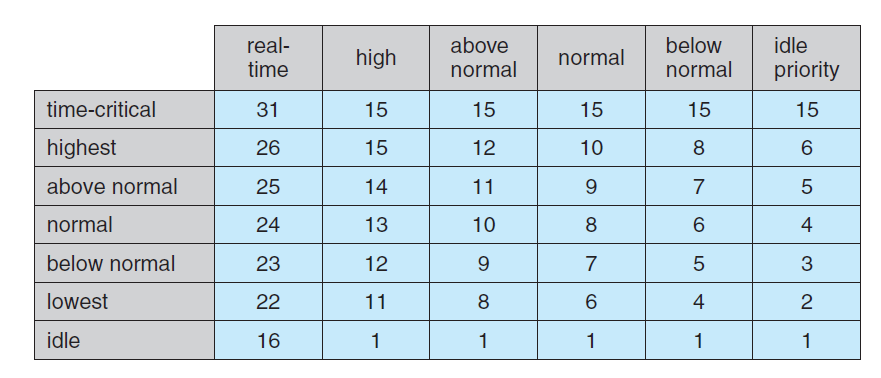
\includegraphics[scale=0.7]{os22.png}
        \caption{Windows Thread Priorities}
        \label{fig:my_label_22}
    \end{figure}
    
    \item When a thread's time quantum runs out, that thread is interrupted. It's priority is lowered if it belongs to a variable priority class.
    
    \item When a variable-pty thread is released from a0\texttt{wait()} operation, its priority is boosted. This is useful for increasing the performance of I/O bound processes, while allowing CPU bound processes to use the spare CPU cycles. 
    
    \item \textbf{User-mode scheduling} introduced in Windows 7 allows user applications to create and manage threads independently of the kernel. Microsoft's \textbf{ConcRT} runtime library for C++ allows user-mode scheduling, user apps to create and manage threads, as well as methods to divide applications into parallelizable tasks. 
\end{itemize}

\section{Interprocess Communication (IPC)}
\begin{itemize}
    \item Processes may be classified as \textbf{independent} (cannot affect or be affected by any other process) or \textbf{cooperative} (can affect/be affected by other processes).
    
    \item Cooperative processes require a method for IPC. The advantages of allowing cooperative processes are 
    \begin{itemize}
        \item Information sharing between users
        
        \item Computation speedup from task-level parallelism 
        
        \item Modularity
        
        \item Convenience due to multitasking
    \end{itemize}
    
    \item The models of IPC are \textbf{shared memory} model and \textbf{message passing} model. \textbf{Pipes} are a model of IPC used in very early UNIX systems, which are not used widely today but are simple to study. 
\end{itemize}

\subsection{Shared Memory Model}
\begin{itemize}
    \item Processes exchange information by writing to and reading from a common memory area dedicated for this task. 
    
    \item The OS normally prevents processes from writing into each other's dedicated memory, but for shared memory IPC this restriction is temporarily removed, upon agreement from both processes. 
    
    
    \item The processes (not OS) control the format of data that is to be shared  as well any coherency issues that arise.
    
\end{itemize}

\subsubsection{Producer-Consumer Problem}
\begin{itemize}
    \item The producer process generates information that is to be read by the consumer process.
    
    \item The solution to this system involves a shared buffer that the producer fills and the consumer empties. The producer may produce an item while the consumer consumes another item in the buffer.
    
    \item The producer and consumer must be synchronized to prevent the consumer from consuming a not-yet generated process. 
    
    \item The following variables are shared by the producer and consumer processes.
    
    \begin{minted}{c}
        #define BUFFER_SIZE 10
        
        typedef struct{
            ...
        }item;
        item buffer[BUFFER_SIZE]; //Buffer array
        int in = 0, out = 0;      //Buffer Pointers
    \end{minted}
    
    \item An \textbf{unbounded buffer} has no size restrictions, thus the producer can produce items indefinitely, but the consumer must wait if the buffer becomes empty at any point.
    
    \item A \textbf{bounded buffer} has a fixed and finite size, hence the consumer must wait if the buffer becomes empty and the producer must wait if the buffer is full. 
    
    \item The buffer is implemented as a circular queue with two pointers \texttt{in} and \texttt{out} at the head and tail respectively. If \texttt{in == out} the queue is empty, and if \texttt{(in + 1)\%BUFFER\_SIZE == out} the queue is full.
\end{itemize}
\begin{figure}[!h]
 \begin{minipage}{0.5\textwidth}
  \centering
  \begin{minted}{c}
   while(true)
   {
    /* Produce an item in next_produced*/
    
        while((in + 1)%BUFFER_SIZE == out)
            ; //Do nothing
        buffer[in] = next_produced;
        in = (in+1)%BUFFER_SIZE;
   }
  \end{minted}
  \title{Producer Process}
 \end{minipage}
 \begin{minipage}{0.5\textwidth}
  \centering
  \begin{minted}{c}
  item next_consumed;
  
  while(true)
   {
        while(in == out)
            ; //Do nothing
        next_consumed = buffer[out];
        out = (out+1)%BUFFER_SIZE;
   }
  \end{minted}
  \title{Consumer Process}
 \end{minipage}
\end{figure}

\subsection{Message Passing}
\begin{itemize}
    \item Allows processes to communicate without sharing a common address space, useful on distributed systems where processes may be connected only by some network. 
    
    \item Every Message Passing interface must provide a \texttt{send(message)} and a \texttt{receive(message)} function. 
    
    \item Messages may have a constant size (easy to implement, hard to write programs using), or a variable size (hard to implement, easy to write programs for). 
\end{itemize}

\subsubsection{Communication}
\begin{itemize}
    \item \textbf{Direct communication} means that processes refer to each other explicitly when sending messages. The processes must know each other's identity if they want to communicate
    
    \item In this scheme, a link is established between every pair of processes that want to communicate. A link is associated withe exactly two processes, and there is only one link between each pair of processes.
    
    \item The direct message passing may be \textit{symmetric} (both sender and receiver name each other explicitly while sending/receiving messages) or \textit{asymmetric} (only sender needs to name the receiver, receiver need not name the sender).
    
    \item Direct communication is not desirable as if a process ID changes then all the message passing calls associated with that process must be changed, which is tedious. 
    
    \item In \textbf{indirect communication}, messages are sent to and received from \textit{mailboxes} or \textit{ports}. 
    
    \item A mailbox may be viewed as an abstract object into which messages can be deposited and from which messages can be retrieved. Mailboxes have their identification numbers (POSIX defines a mailbox ID), and two processes can communicate only if they have a shared mailbox. 
    
    \item If process $P_1$ sends a message to mailbox $M$, and processes $P_2$ and $P_3$ execute a \texttt{receive()} call from mailbox $M$ at the same time, this leads to concurrency issues. These are resolved using any one of the following
    \begin{itemize}
        \item Allow one link between 2 fixed processes only
        
        \item Allow only one process to execute a \texttt{receive()} call at a time
        
        \item Allow the system to use an algorithm to identify the next receiver (such as a round robin system)
    \end{itemize}
    
    \item A mailbox may be owned by a process or the OS. If the process owns the mailbox, then it can only receive from that box, while other processes can only send to that mailbox.
    
    \item If the OS owns the mailbox, then it must provide a means to create, delete mailboxes and a message passing interface. 
\end{itemize}

\subsubsection{Synchronization}
\begin{itemize}
    \item \textbf{Blocking send}: The process that sends is blocked until the message currently being sent is received and read by the receiver or the receiving mailbox. 
    
    \item \textbf{Non-blocking Send}: Sending process can send a message and resume operation.
    
    \item \textbf{Blocking receive}: The receiver process blocks itself until a message arrives.
    
    \item \textbf{Non-blocking receive}: The receiver retrieves either a valid message or a NULL message.
    
    \item When both send and receive are blocking, there is a \textbf{rendezvous} between the two processes. This makes the solution to the producer-consumer problem trivial. 
\end{itemize}

\subsubsection{Buffering}
\begin{itemize}
    \item All messages are stored in a temporary queue as they travel from sender to receiver. This queue can be implemented as:
    
    \begin{itemize}
        \item \textbf{Zero-capacity} buffer: The link cannot have any messages waiting in it, hence the sender must block itself until the current message is received. 
        
        \item \textbf{Bounded} buffer: The sender can continue to work after it sends the message, but if the queue is full then the sender must block itself until the queue has space again. 
        
        \item \textbf{Unbounded} buffer: The sender is never required to block itself, it can send an infinite amount of messages and resume operation.
    \end{itemize}
\end{itemize}

\begin{figure}[!h]
 \begin{minipage}{0.5\textwidth}
  \centering
  \begin{minted}{c}
   message next_produced;
   while(true)
   {
        //Produce a message
        next_produced = produce_message();
        send(next_produced);
   }
  \end{minted}
  \title{Sender Process}
 \end{minipage}
 \begin{minipage}{0.5\textwidth}
  \centering
  \begin{minted}{c}
  message next_consumed;
  while(true)
   {
        receive(next_consumed);
        /* Consume this message */
        consume(next_consumed);
   }
  \end{minted}
  \title{Receiver Process}
 \end{minipage}
\end{figure}

\subsection{Pipes}
\begin{itemize}
    \item Pipes are the simplest form of IPC, found in the earlier UNIX systems.
    
    \item The considerations while implementing pipes are whether
    \begin{itemize}
        \item The pipe allows bidirectional communication?
        
        \item If it does, is it half duplex or full duplex?
        
        \item Must a relationship (eg: parent-child) exist between the processes?
        
        \item Can the processes be on different machines (comm. over  a network) or must they be on the same machine?
    \end{itemize}
\end{itemize}

\subsubsection{Ordinary Pipes}
\begin{itemize}
    \item Ordinary pipes are unidirectional, allowing only one-way communication.
    
    \item The producer writes to the \textbf{write-end} of the pipe, while the consumer reads from the \textbf{read-end} of the pipe. 
    
    \item Ordinary pipes in UNIX are constructed using the \texttt{pipe(int fd[])} function, where the array \texttt{fd} holds the file descriptors of the read end (index 0) and write end (index 1).
    
    \item UNIX treats pipes as a special type of file, hence pipes can be accessed using the \texttt{read()} and \texttt{write()} system calls.
    
    \item Ordinary pipes require a parent-child relationship between the processes, hence the processes must be on the same machine
    
    \item Once the processes finish communicating and terminate, the named pipe ceases to exist.
\end{itemize}

\subsubsection{Named Pipes}
\begin{itemize}
    \item These allow bidirectional communication, and no parent-child hierarchy is needed between the communicating processes. 
    
    \item Several processes can use a single named pipe, and a named pipe typically has several writers. 
    
    \item The named pipe is retained in the memory even after all the communicating processes terminate, and it stays that way until it is explicitly deleted. 
    
    \item UNIX named pipes allow only half duplex communication, and all processes must be on the same machine. They are referred to as FIFOs, they are created by the \texttt{mkfifo()} system call, and accessed using the \texttt{open()}, \texttt{read()}, \texttt{write()} and \texttt{close()} system calls.
    
    \item Windows named pipes allow full duplex communication, inter machine communication and transfer of both byte- and message-oriented data. 
\end{itemize}
\end{document}

